\section{Integration Strategy}

\subsection{Entry Criteria}
\label{sec:entryCriteria}
The following conditions have to be verified before entering the integration testing phase in order for it to produce meaningful results.\\

A fundamental initial criterion is that the development of the components and their functionalities proceeds together with the unit testing on such components, so that even when the components are not fully developed, they have already been tested at unit level w.r.t. the fully developed functionalities. 
Given the aforementioned criterion, before entering the integration phase, the development percentage of a component must be at least 90\% and the main functionalities required to test its integration w.r.t. another component of the system must be fully developed.\\

The integration process can start when these conditions are met by the system development
\begin{itemize}
	\item 100\% of development on the \emph{Data Provider} component
	\item 90\% of development on the \emph{Event Broker} and \emph{Car Handler} components
	\item 80\% of development on the \emph{Rent Manager} component
	\item 60\% of development on the \emph{Maintenance Manager} component
	\item 40\% of development on the \emph{User Information Manager} and \emph{Access Manager} components
	\item 30\% of development on the \emph{User Application Server}, \emph{User Application}, \emph{Customer Care Server} and \emph{Customer Care Application} components
\end{itemize}

\subsection{Elements to be integrated}
In this section we identify the components and subcomponents to be integrated and add some details about their specific integration.\\

As specified in the design document, some component of the PowerEnJoy system such as the \emph{Rent Manager} and the \emph{Maintenance Manager} are rather complex and thus its internal subcomponents need to be integrated before proceeding with the integration of entire components with other components of the system.\\

The following components will be integrated to obtain the subsystem related to the Maintenance functionalities:

\begin{itemize}
	\item \emph{Maintenance Manager}
	\item \emph{Event Broker}
	\item \emph{Data Provider}
	\item \emph{Car Handler}
\end{itemize}

The following components will be integrated to obtain the subsystem related to the User Application functionalities:

\begin{itemize}
	\item \emph{User Application}
	\item \emph{UserApp Server}
	\item \emph{Access Manager}
	\item \emph{Rent Manager}
	\item \emph{User Information Manager}
	\item \emph{Data Provider}
	\item \emph{Car Handler}
	\item \emph{Event Broker}
\end{itemize}

The following components will be integrated to obtain the subsystem related to the Customer Care functionalities:

\begin{itemize}
	\item \emph{Customer Care Application}
	\item \emph{Customer Care Server}
	\item \emph{User Information Manager}
	\item \emph{Data Provider}
\end{itemize}

\paragraph{Notes}
The external components like the \emph{DBMS} and the external APIs are products that are not developed by us and that we suppose already completely tested; however we decided to include them in the integration testing by firstly testing the external component's interfaces on their own, and the by proceeding to test them when integrated with PowerEnJoy components.\\
In the same way the Maintenance Manger will be tested as a component integrated with our system and then it will be tested through the Maintenance API it provides to the maintenance company. 

\subsection{Integration Testing Strategy} \label{sec:intStrategy}
Both bottom-up and top-down were taken in consideration when thinking of the integration strategy for the PowerEnJoy system; looking at the structure and composition of the system it is clear the most complex and relevant functionalities are located in the lower end tiers, which are also the most independent ones. Moreover as stated in \hyperref[sec:entryCriteria]{Section 2.1} those will be the only fully developed components at the time of starting the integration process since the software development of the PowerEnJoy system will proceed using the bottom-up approach. These considerations brought us to lean towards a bottom-up approach that will allow the lower end components to be tested and integrated before any other component; doing so any issue or problem in the integration phase of these components will be found at an early stage in the integration process, and so it will be easier to tackle it and solve it, while maintaining as much parallelism and decoupling as possible.\\
Given that some functionalities of the system are decoupled, during the integration process some steps of the integration sequence will have the same priority. In those cases the critical-module-first approach will be used in order to integrate and test the riskiest  components first and solve their issues before they create worse problems in the integration process.

\subsection{Sequence of Component Integration}
This section describes the proposed plan for the integration test phase of the PowerEnJoy system.

\subsubsection{Overall Component Integration Diagram}  \label{sec:overallPrecedences}
The diagram above shows the needed precedences in the integration phase between the main components of the system taking into account the integration testing strategy chosen.

\paragraph{NOTES} In the following diagram we represent with arrows the precedences needed between the components, the purpose is to indicate that following the strategy chosen a component can be integrated with another one only if that component has already been integrated with all the components it needs to be integrated with (arrows point from the \emph{<need integration>} component to the \emph{<needed integration>} one, numbers are shown to clearify order of the integration and steps that are possibly made in parallel).\\


	\begin{figure}[h]
			\centering
			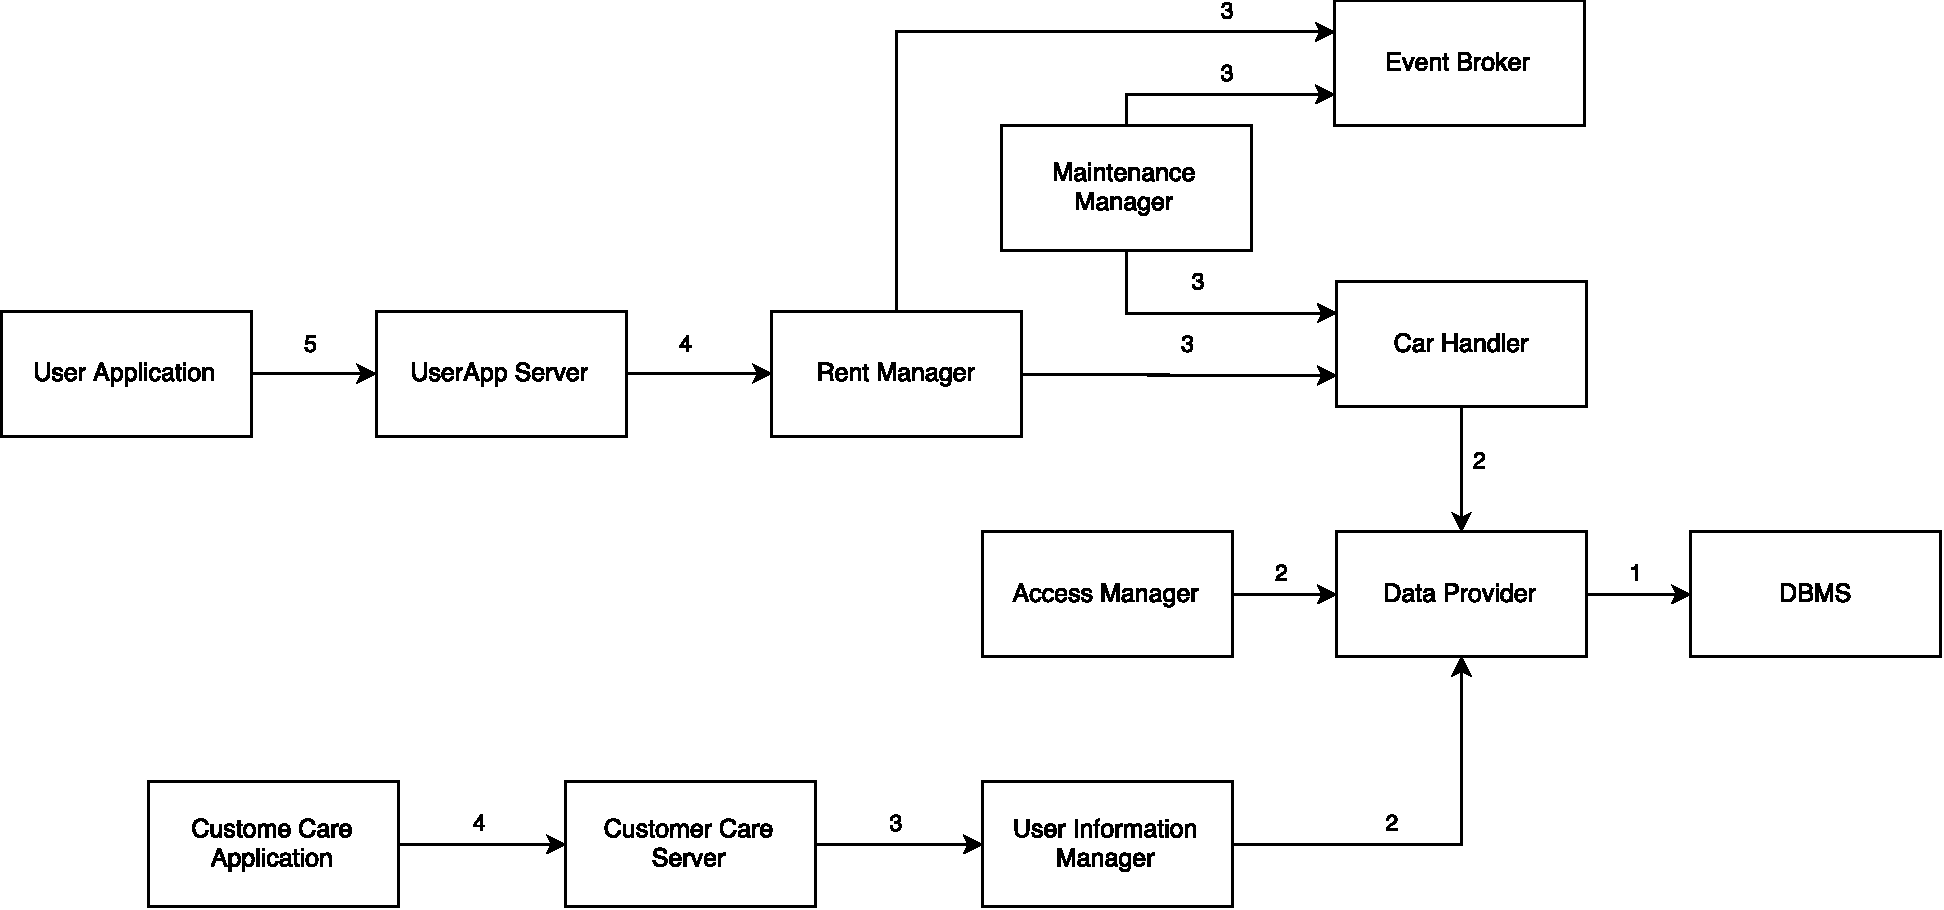
\includegraphics[width=\linewidth]{img/overallIntegration}
			\caption{
				\label{fig:overallIntegration} 
				\emph{Overall Component Integration Diagram}
			}
	\end{figure}
	
\clearpage
\subsubsection{Subcomponent Integration}
In the \emph{PowerEnJoy: Design Document}\cite{DD} some high-level components are described deeply through the definition of the subcomponents composing them.
In this section are shown the diagram of the precedences between the subcomponents to integrate them. We assume that when the high-level component enters the integration sequence presented they have been fully tested inside considering them as a single component unit-level tested to be integrated.

\paragraph{RentManager} 
The diagram above shows the needed precedences in the integration phase between the \emph{RentManager} subcomponents.
\paragraph{}

		\begin{figure}[h]
			\centering
			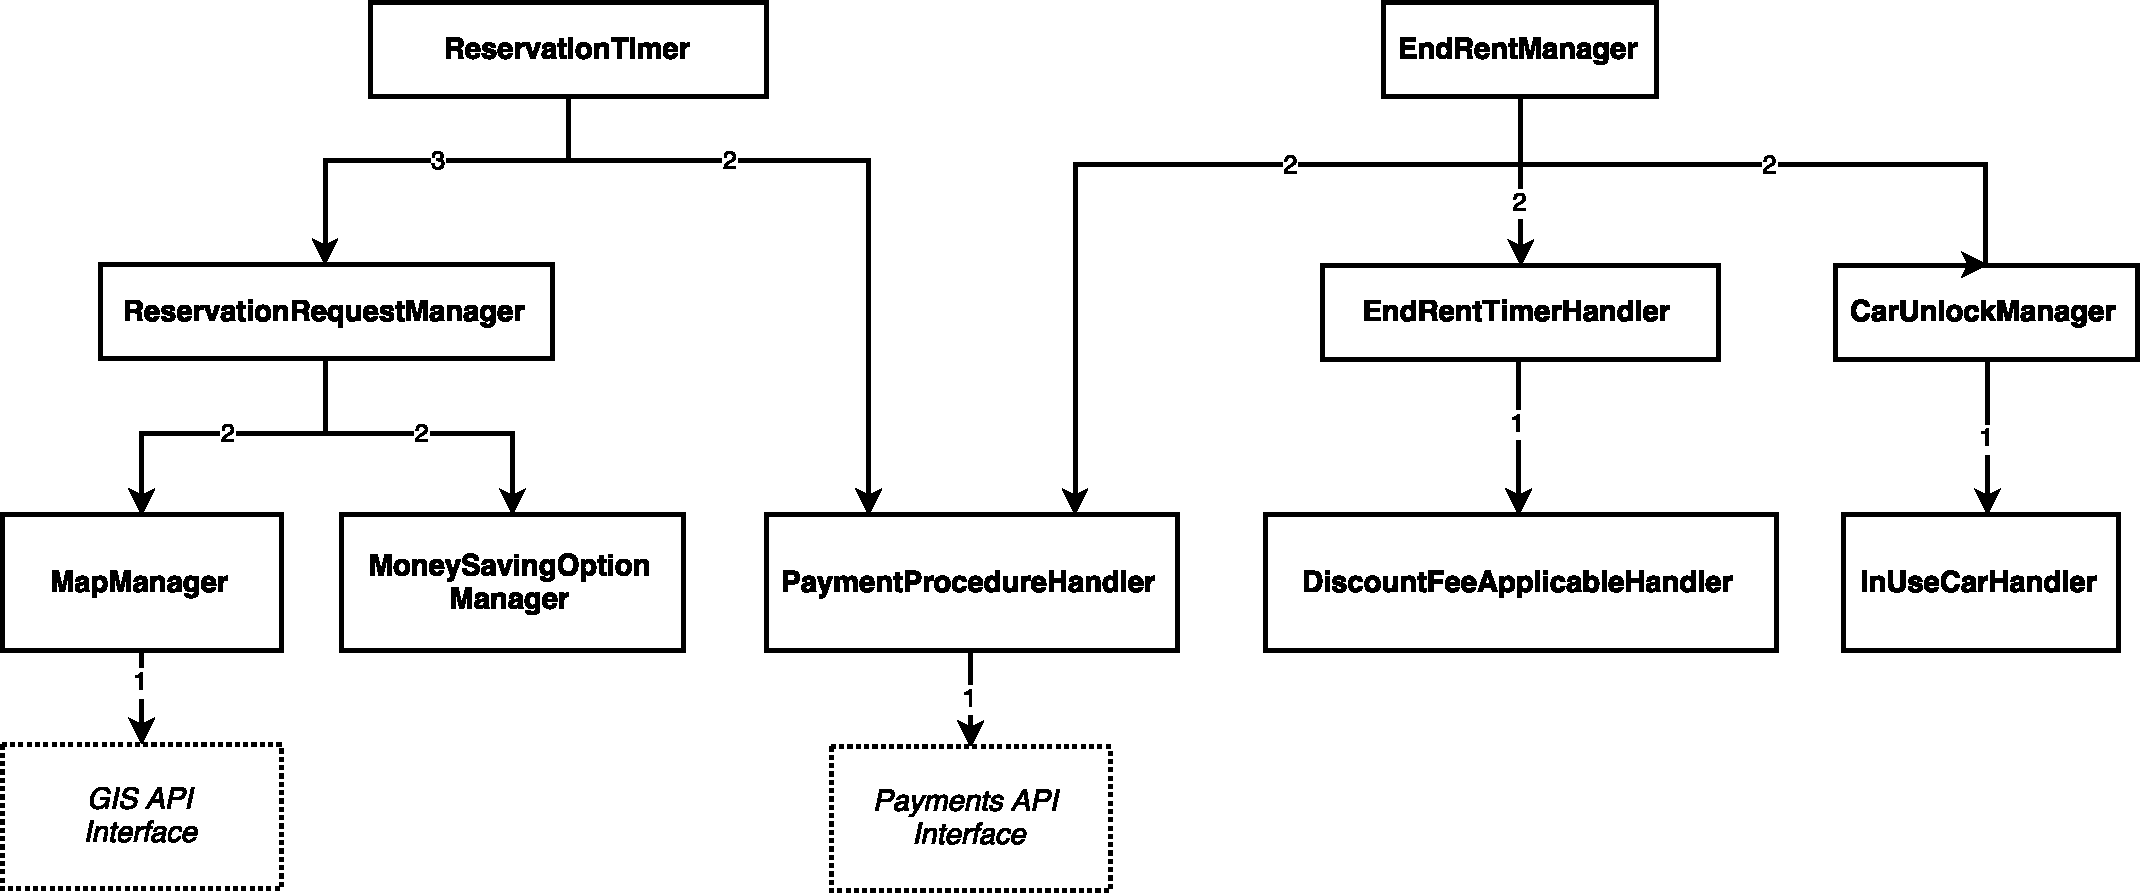
\includegraphics[width=\linewidth]{img/rentManagerIntegration}
			\caption{
				\label{fig:rentManagerIntegration} 
				\emph{RentManager subcomponents integration}
			}
		\end{figure}
		
\paragraph{MaintenanceManager} 
The diagram above shows the needed precedences in the integration phase between the \emph{MaintenanceManager} subcomponents.
\paragraph{}

		\begin{figure}[h]
			\centering
			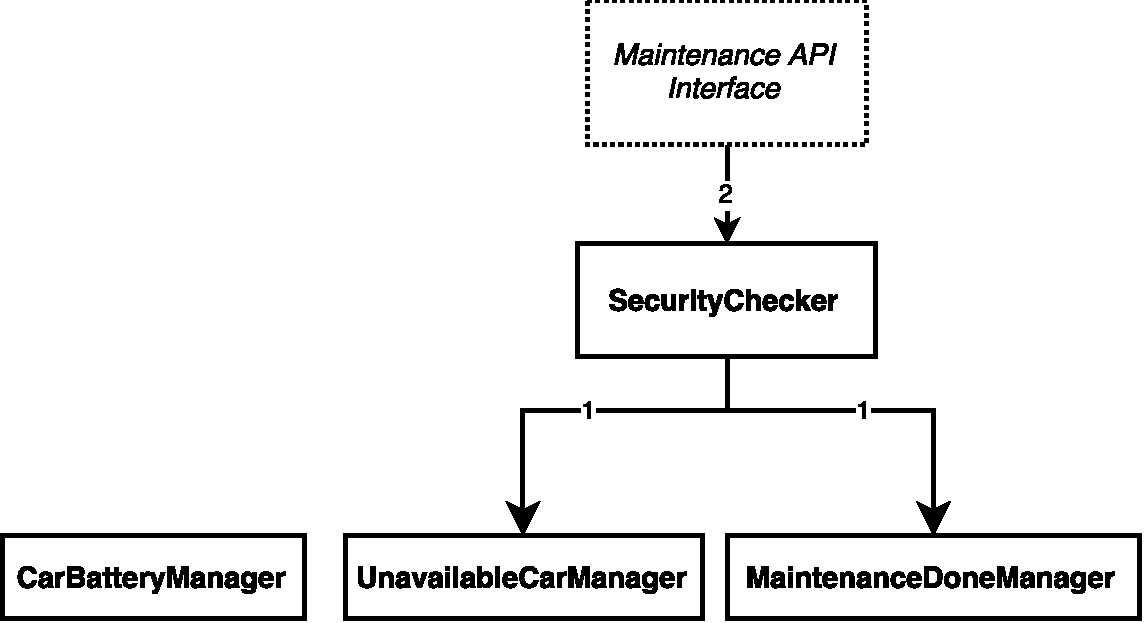
\includegraphics[width=0.6\linewidth]{img/maintenanceIntegration}
			\caption{
				\label{fig:maintenanceIntegration} 
				\emph{MaintenanceManager subcomponents integration}
			}
		\end{figure}
		
\paragraph{UserInformationManager} 
The diagram above shows the needed precedences in the integration phase inside the \emph{UserInformationManager} subcomponents.
\paragraph{}

		\begin{figure}[h]
			\centering
			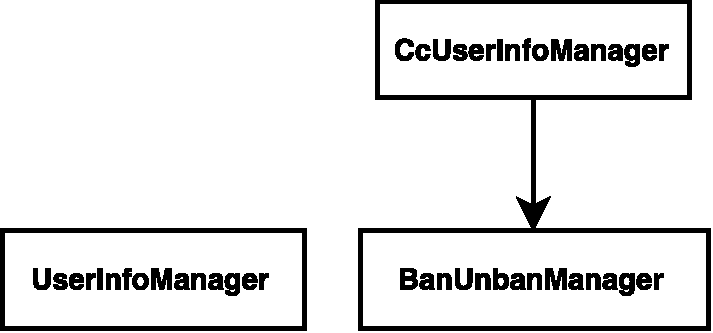
\includegraphics[width=0.4\linewidth]{img/userIntegration}
			\caption{
				\label{fig:userIntegration} 
				\emph{UserInformationManager subcomponents integration}
			}
		\end{figure}

\clearpage 

\subsubsection{Component Integration}
This section describes the sequence proposed to plan the integration test of all the components of the PowerEnJoy system. As specified in the \hyperref[sec:intStrategy]{Integration Testing Strategy section} we decide to start the bottom-up integration from the components related to the critical functionalities of the system (such as the communication with cars); even if the steps are proposed sequentially following these criteria, it is clear the sequence proposed presents the possibility to make same integration steps in parallel given the needed precedences between components presented in the \hyperref[sec:overallPrecedences]{Overall Component Integration Diagram}.

\paragraph{DataProvider} 
The first step of our integration sequence is to integrate the \emph{DataProvider} component with the DBMS component.
\paragraph{}

		\begin{figure}[h]
			\centering
			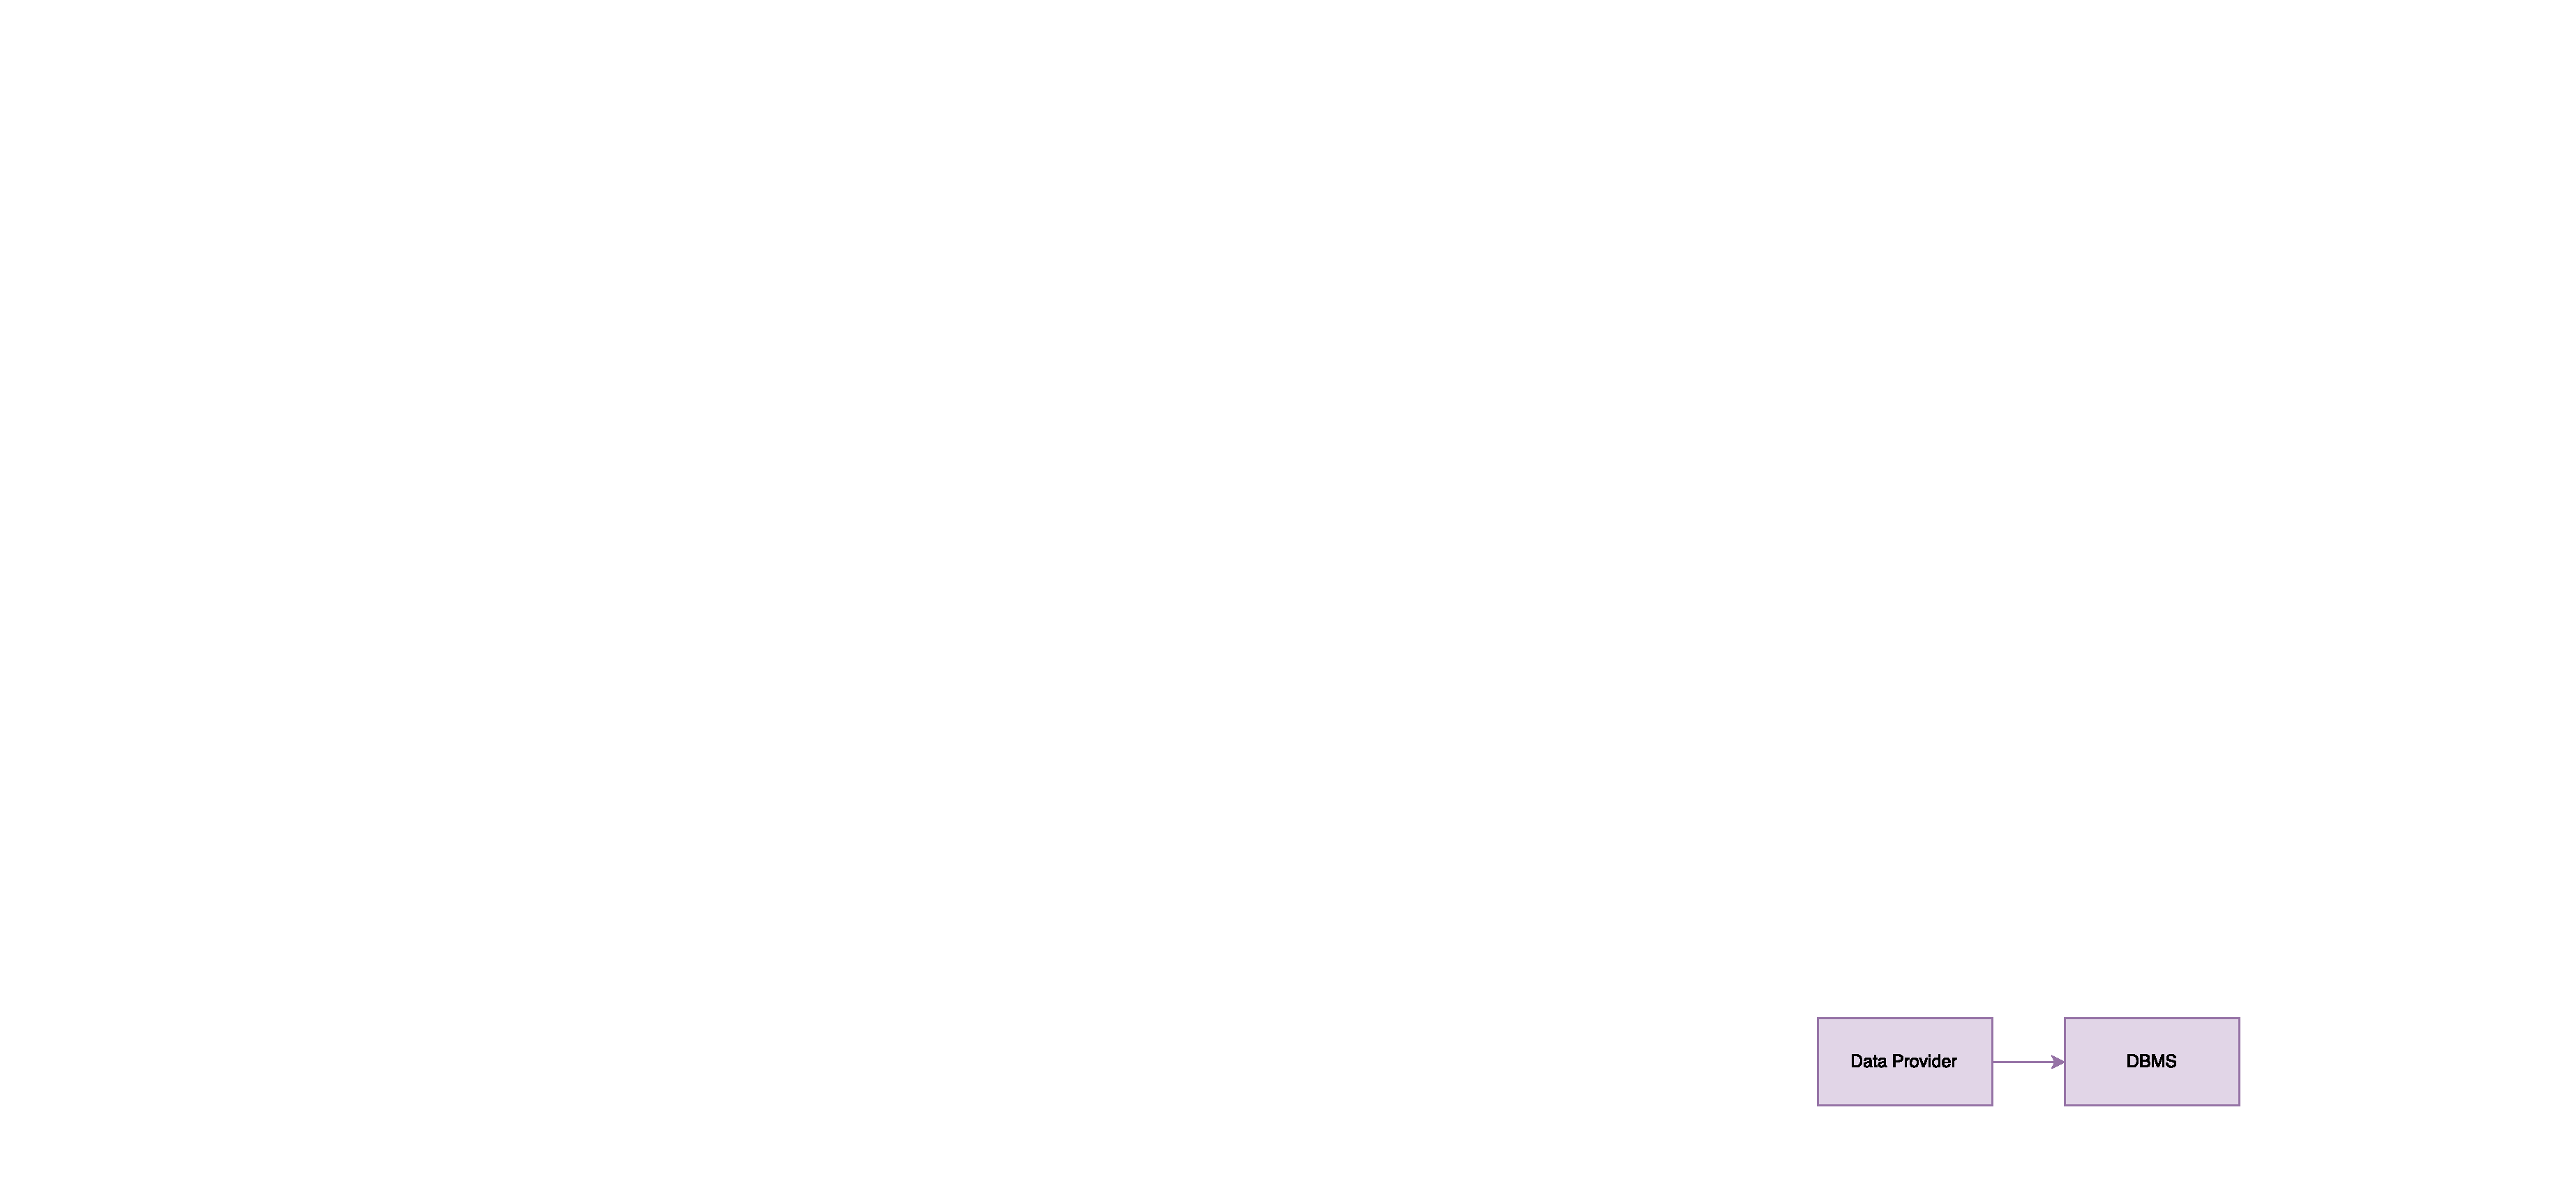
\includegraphics[width=0.6\linewidth]{img/Integration1}
			\caption{
				\label{fig:dataProvider} 
				\emph{DataProvider integration}
			}
		\end{figure}

\paragraph{EventBroker and CarHandler} 
After that we integrate the \emph{EventBroker} and the \emph{CarHandler} with the external API provided by the car embedded system testing the interfaces between our system and them. We also integrate the \emph{CarHandler} with the {DataProvider} component.\\
\paragraph{}
		
		\begin{figure}[h]
			\centering
			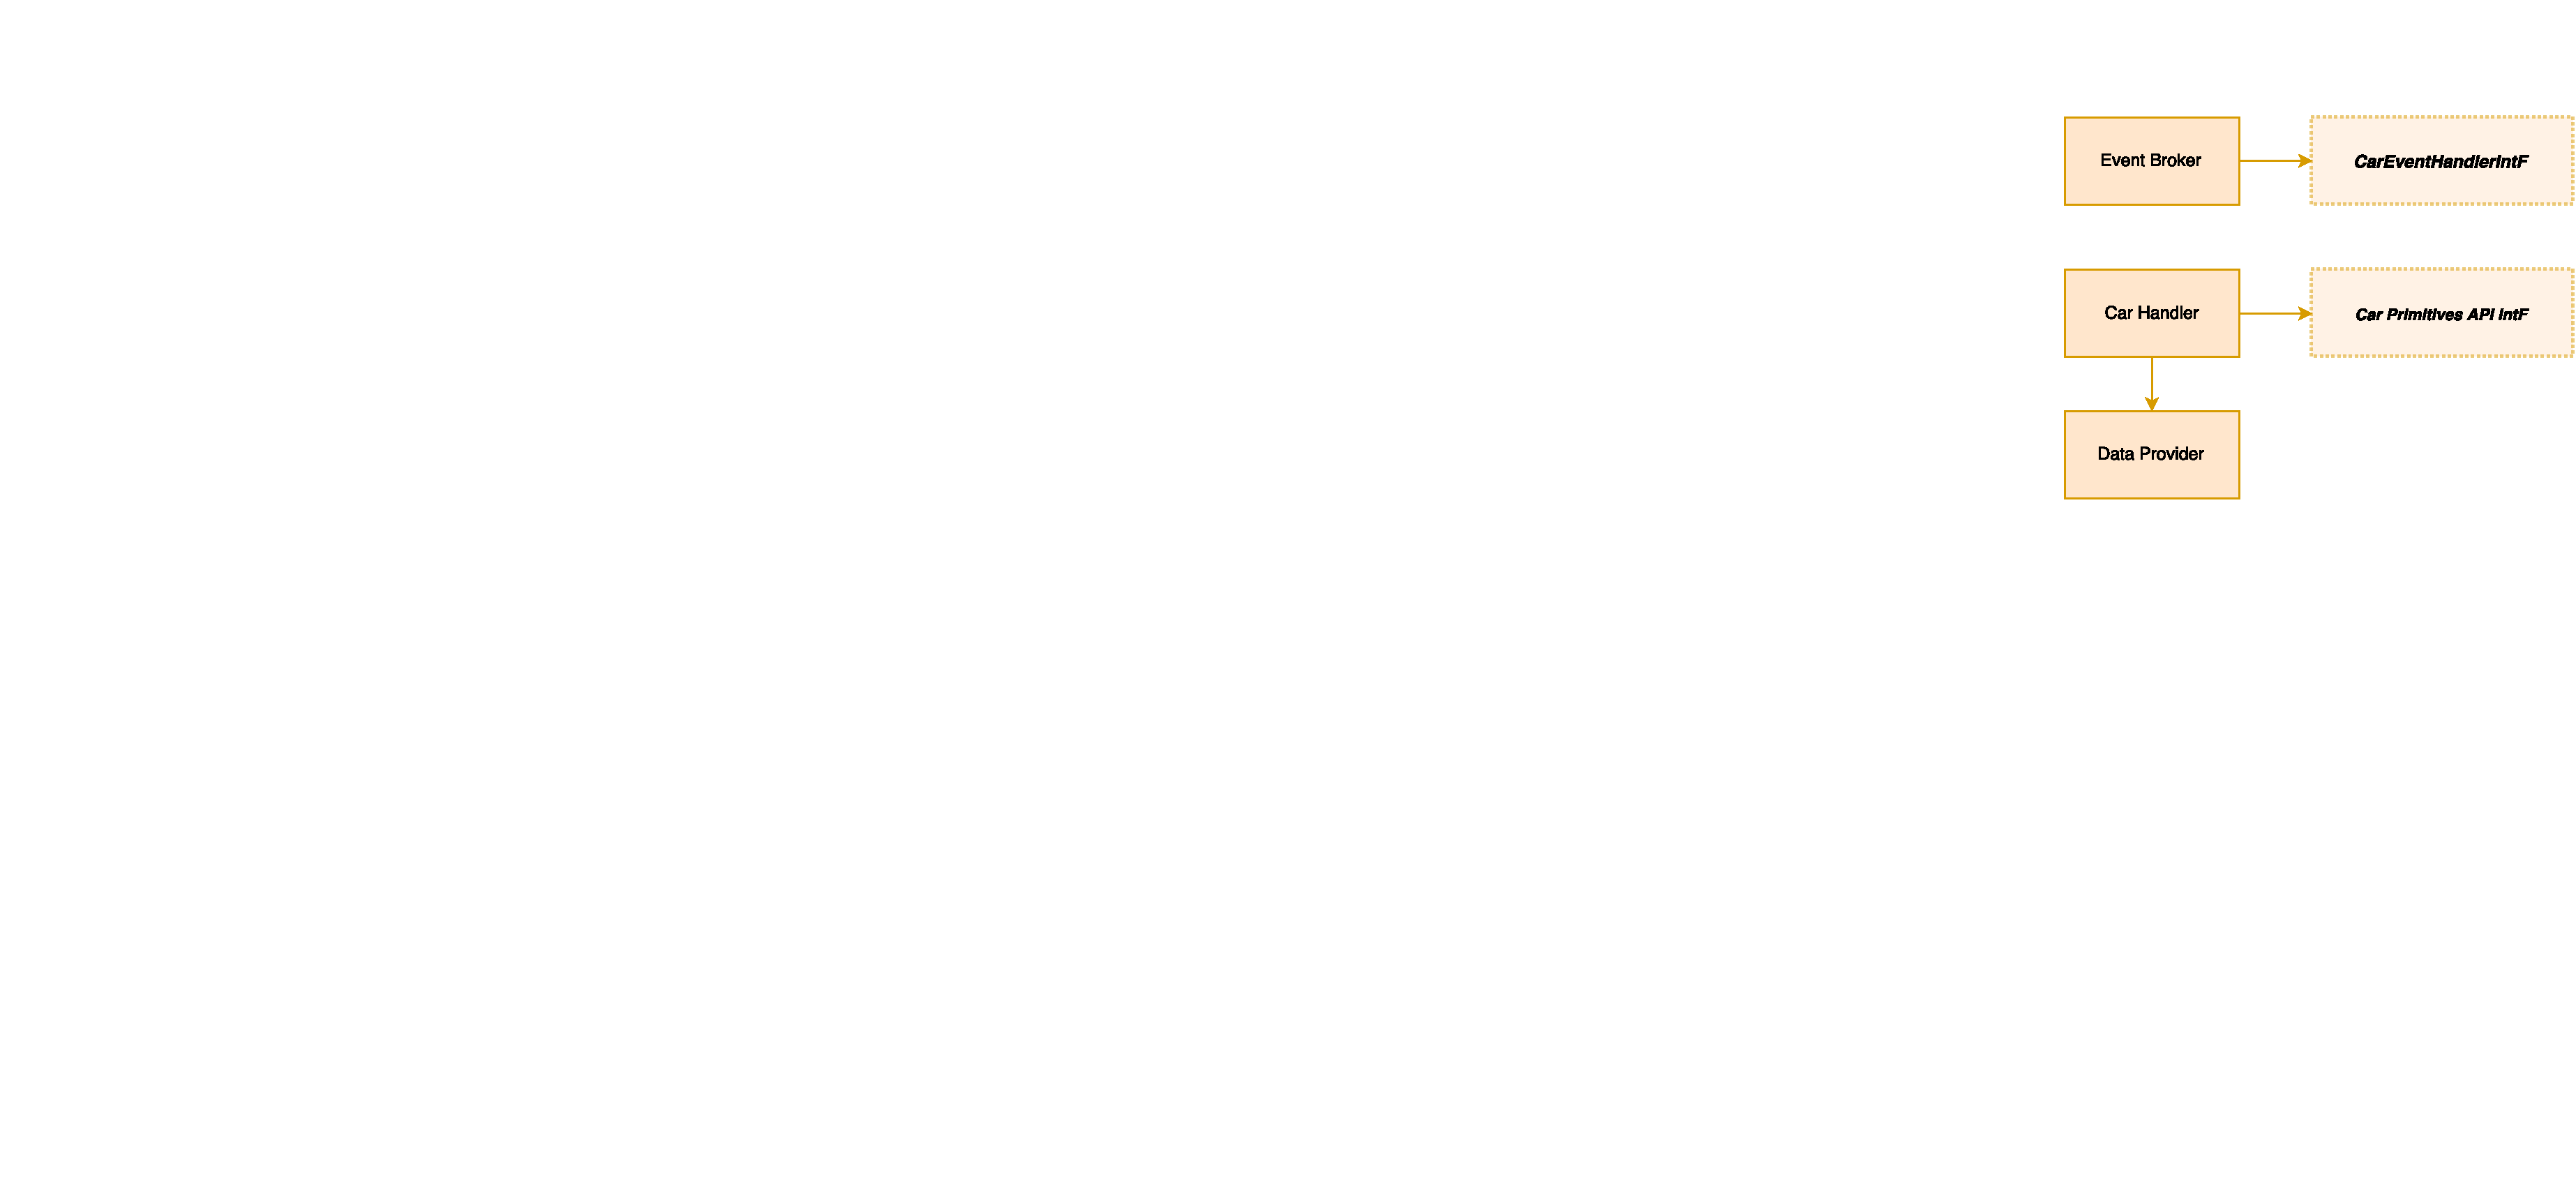
\includegraphics[width=0.6\linewidth]{img/Integration2a}
			\caption{
				\label{fig:eventBrokerCarHandler} 
				\emph{EventBroker and CarHandler integration}
			}
		\end{figure}

\clearpage
\paragraph{UserInformationManager and AccessManager} 
The integration between the \emph{UserInformationManager} and the \emph{DataProvider} components and between the \emph{AccessManager} and the \emph{DataProvider} components are here reported because they can be made at this point of the sequence (given the integration tests already completed), however it is suggested to first complete the critical integration of the \emph{RentManager} component. \\
\paragraph{}
		
		\begin{figure}[h]
			\centering
			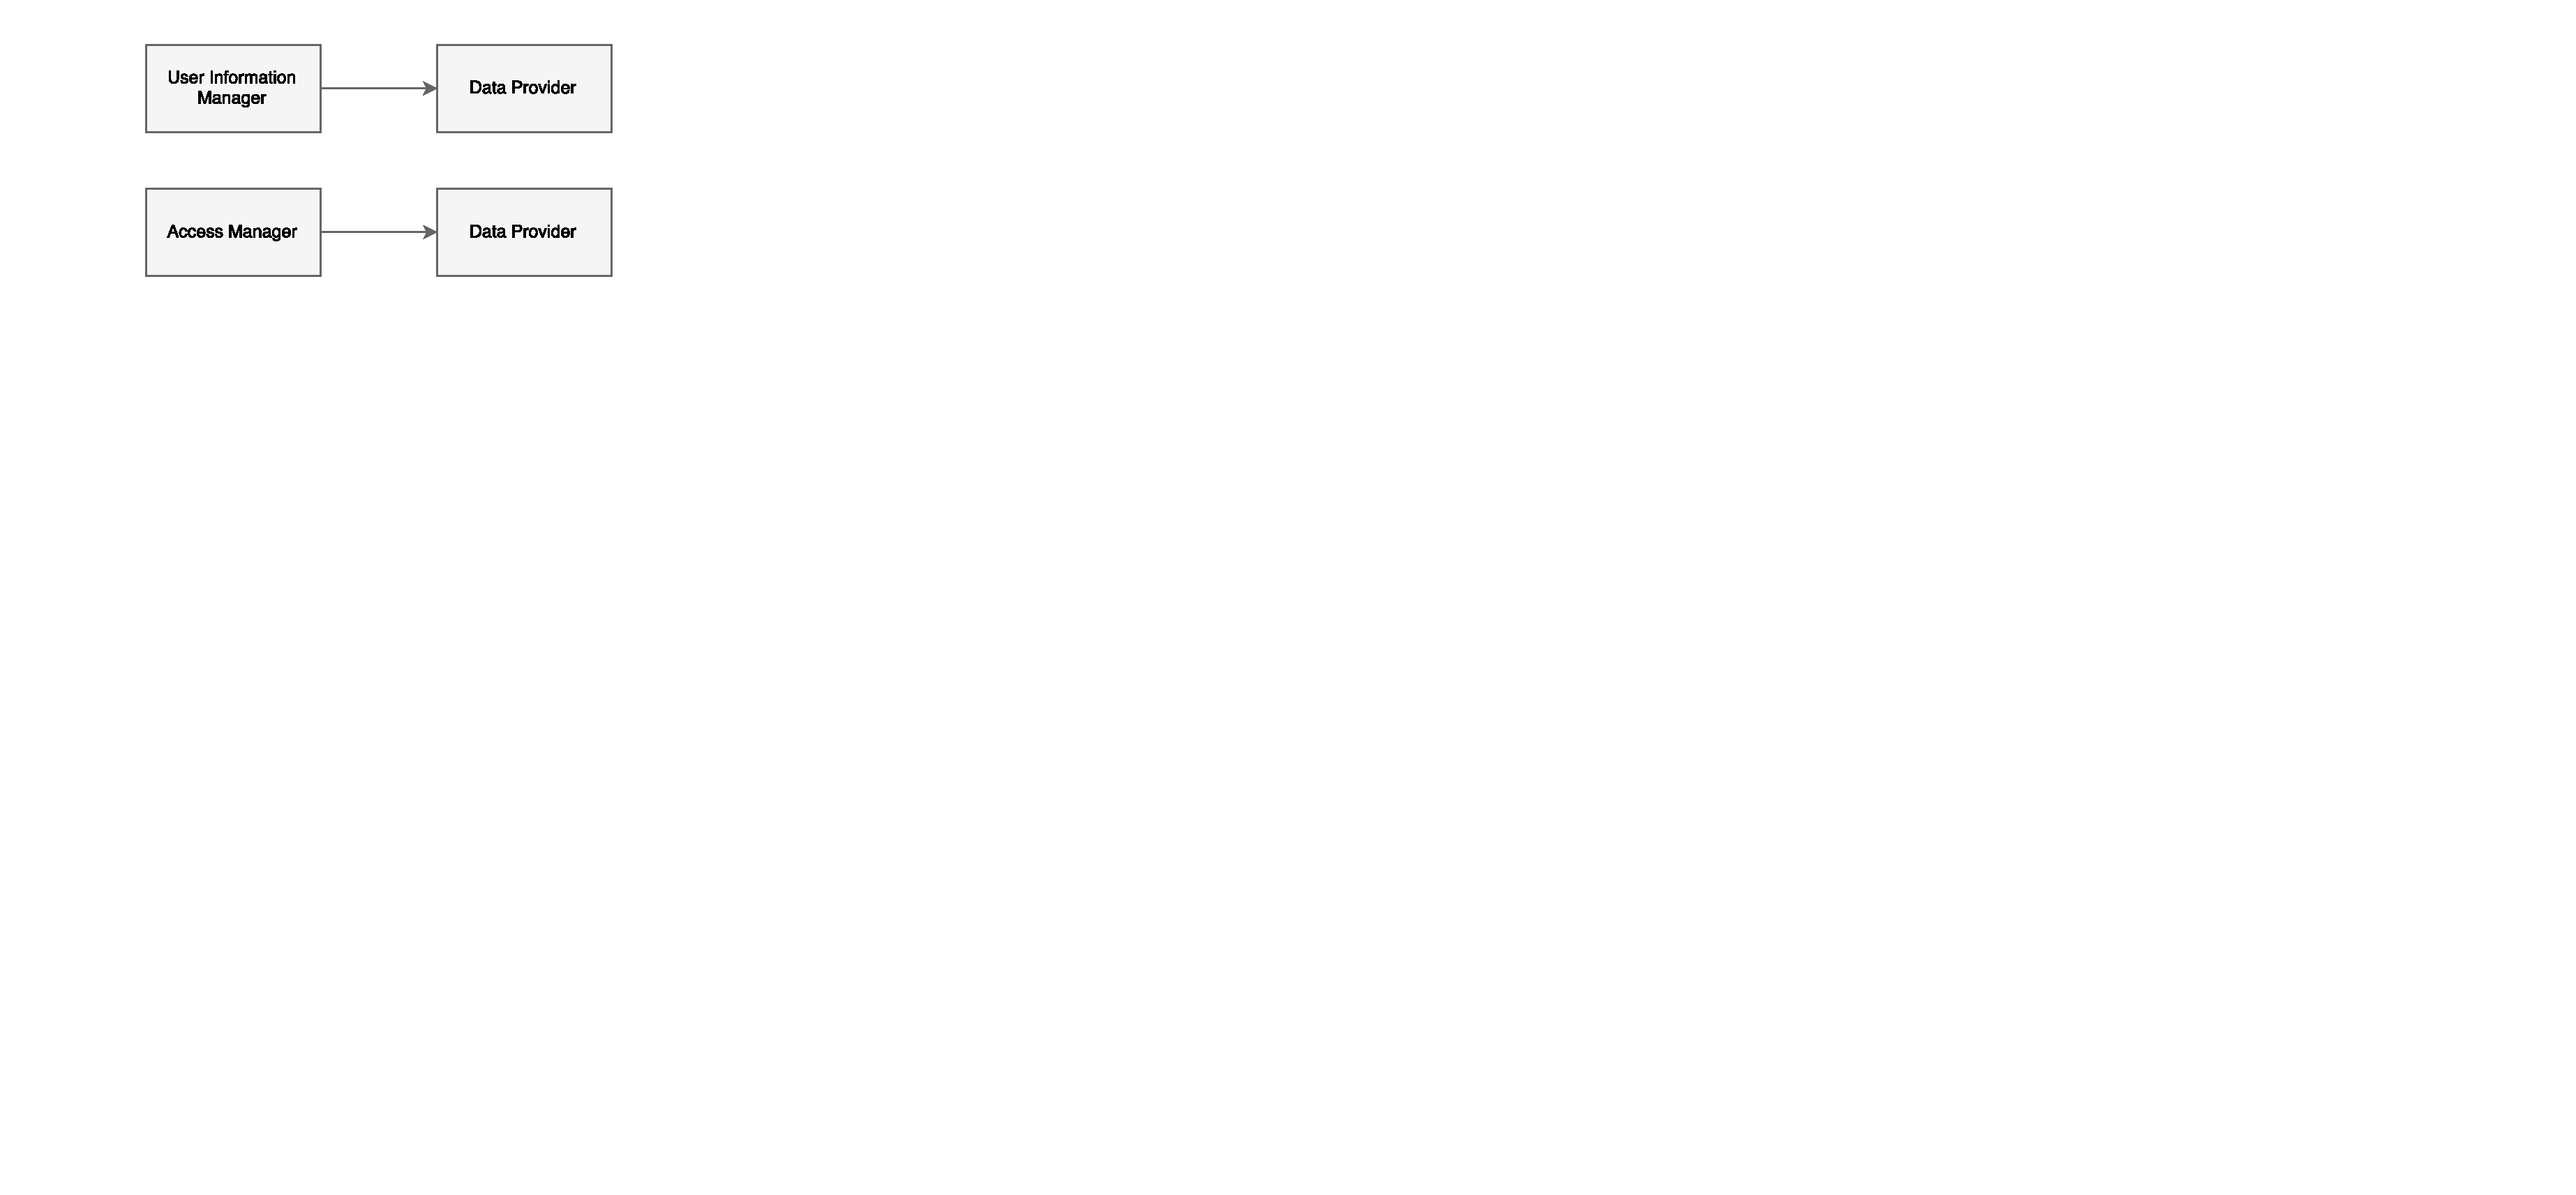
\includegraphics[width=0.5\linewidth]{img/Integration2b}
			\caption{
				\label{fig:userInfoAccessManager} 
				\emph{UserInformationManager and AccessManager integration}
			}
		\end{figure}
		
\paragraph{RentManager} 
After that we integrate the \emph{EventBroker}, the \emph{CarHandler} and the \emph{DataProvider} with the \emph{RentManager}. We also integrate the \emph{RentManager} component with the external APIs related to the GIS and the Payment System testing the interfaces between our system component and them. This integration step is really critical to the functionality provided by our system and a lot of care must be given in the integration tests of the \emph{RentManager} on the communication with cars and the consistency between information provided by cars and information in our database.  \\
\paragraph{}
		
		\begin{figure}[h]
			\centering
			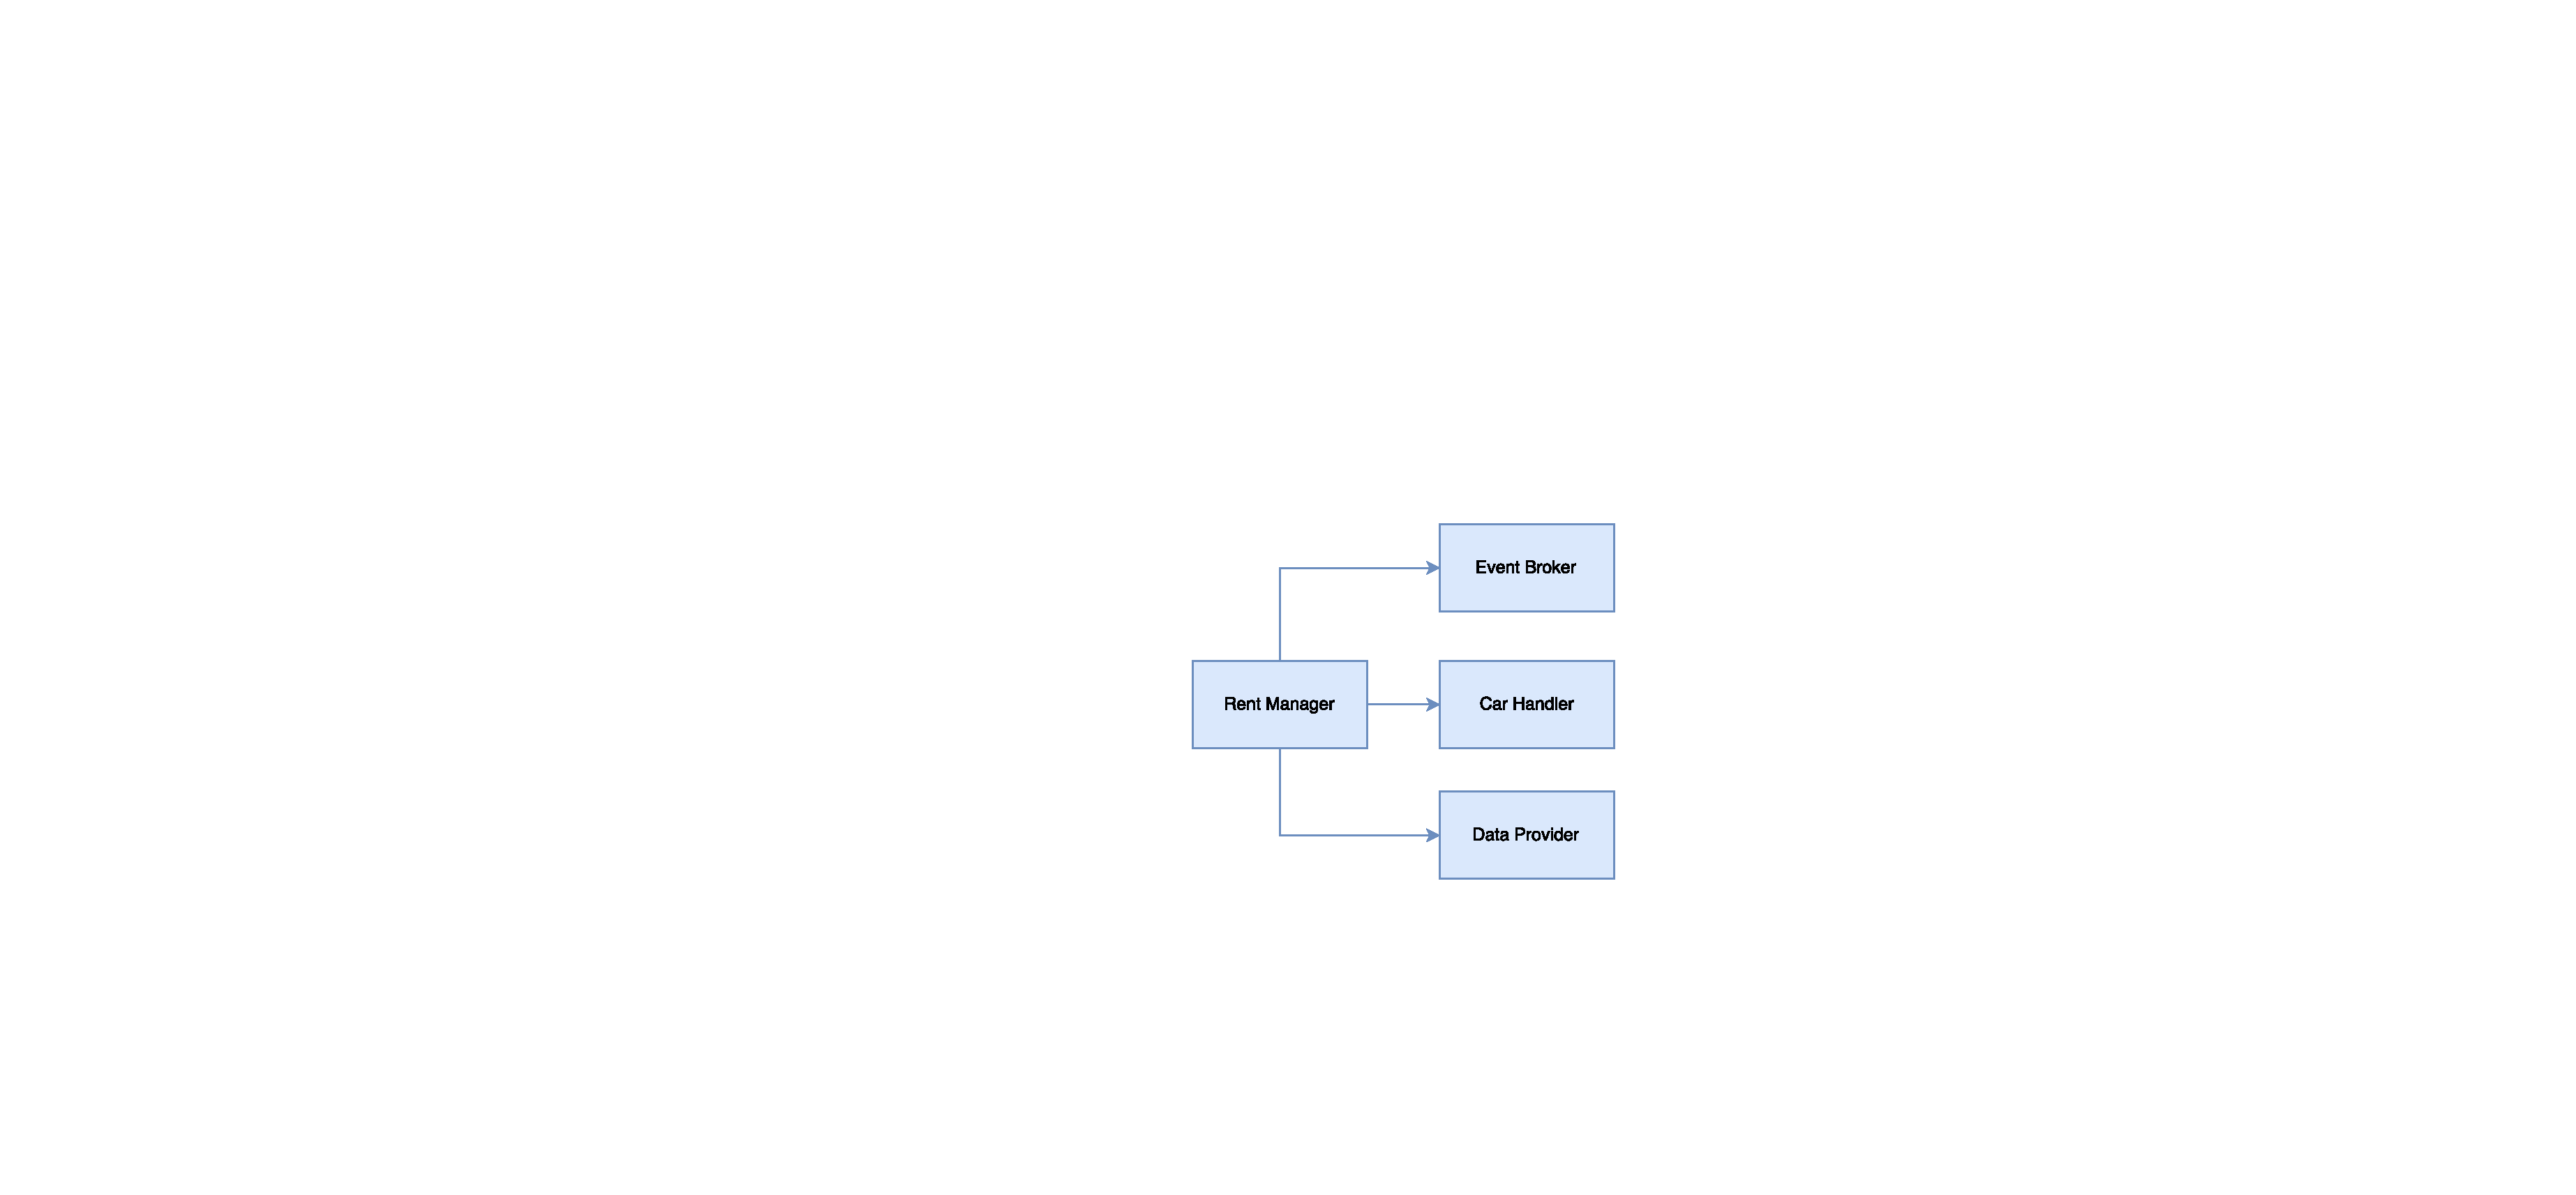
\includegraphics[width=0.8\linewidth]{img/Integration3a}
			\caption{
				\label{fig:rentManager} 
				\emph{RentManager integration}
			}
		\end{figure}

\paragraph{MaintenanceManager} 
After that we integrate the \emph{EventBroker}, the \emph{CarHandler} and the \emph{DataProvider} with the \emph{MaintenanceManager} obtaining the complete test of the subsystem related to the functionalities to manage the maintenance API. We also want to test the integration between the maintenance subsystem and the API interface exposed externally checking the token mechanism (\emph{see \cite{DD} for more details}) and its correctly behaviour for a "user" external to the system.
\paragraph{}
		
		\begin{figure}[h]
			\centering
			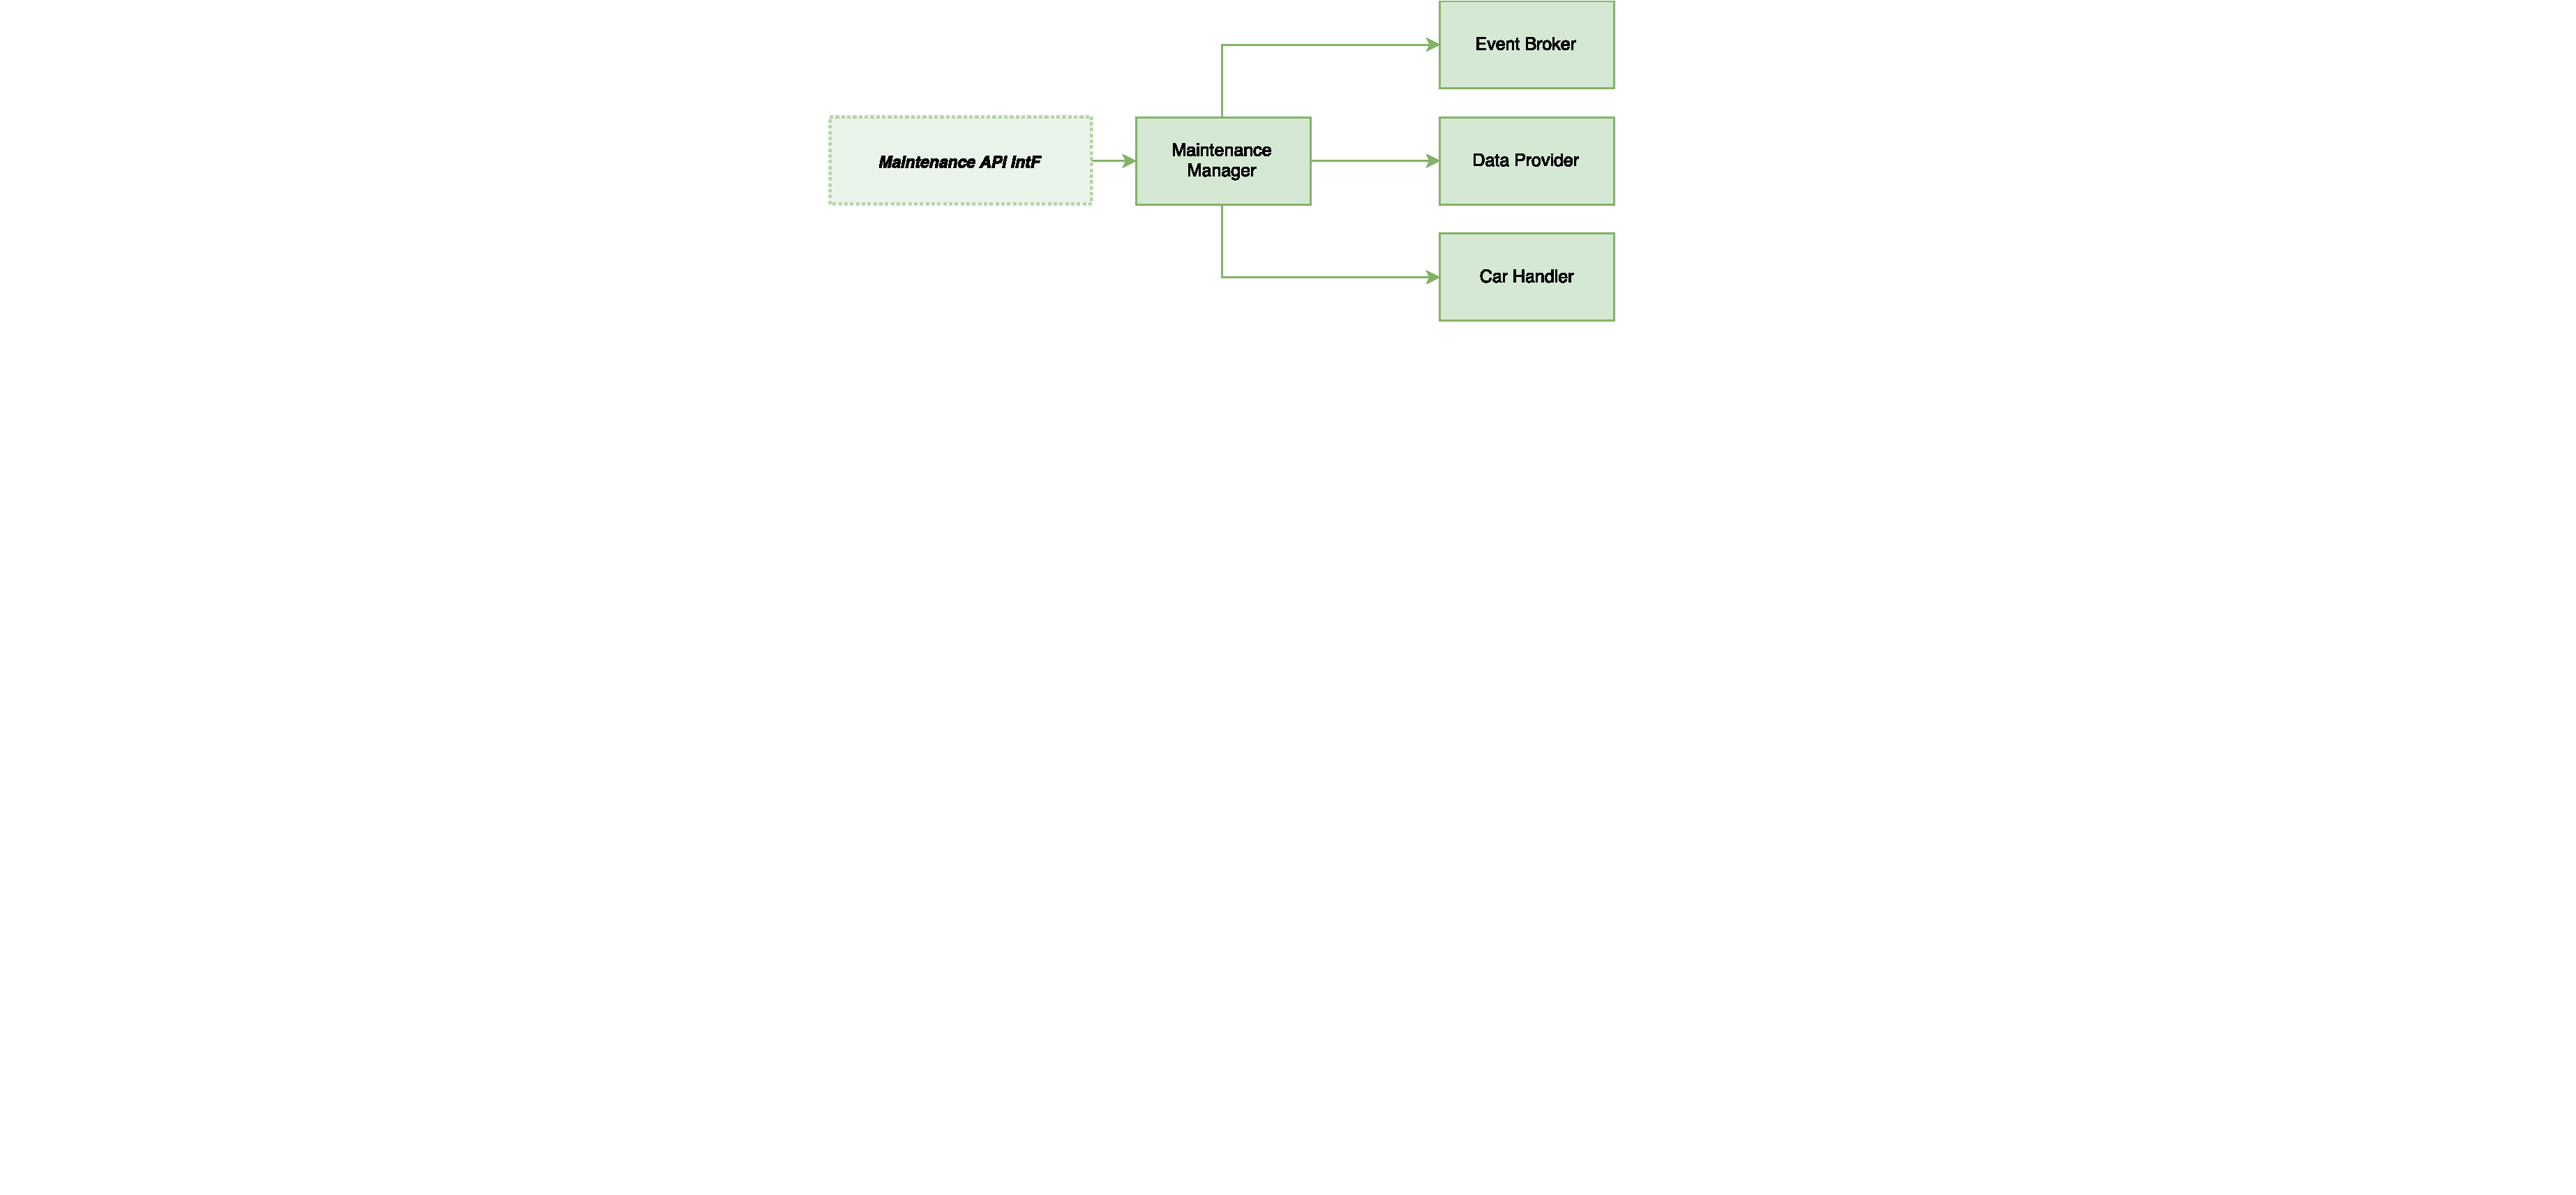
\includegraphics[width=0.8\linewidth]{img/Integration3b}
			\caption{
				\label{fig:maintenanceManager} 
				\emph{MaintenanceManager integration}
			}
		\end{figure}
		
\paragraph{User Application and Server} 
After that, we first integrate the \emph{UserAppServer} with the \emph{AccessManager}, \emph{RentManager} and \emph{UserInformationManager}components and secondly we test the integration between the \emph{UserAppServer} and the \emph{UserApplication} obtaining the complete test of the subsystem related to the functionalities provided to a user of the \emph{Power EnJoy system}.
\paragraph{}
		
		\begin{figure}[h]
			\centering
			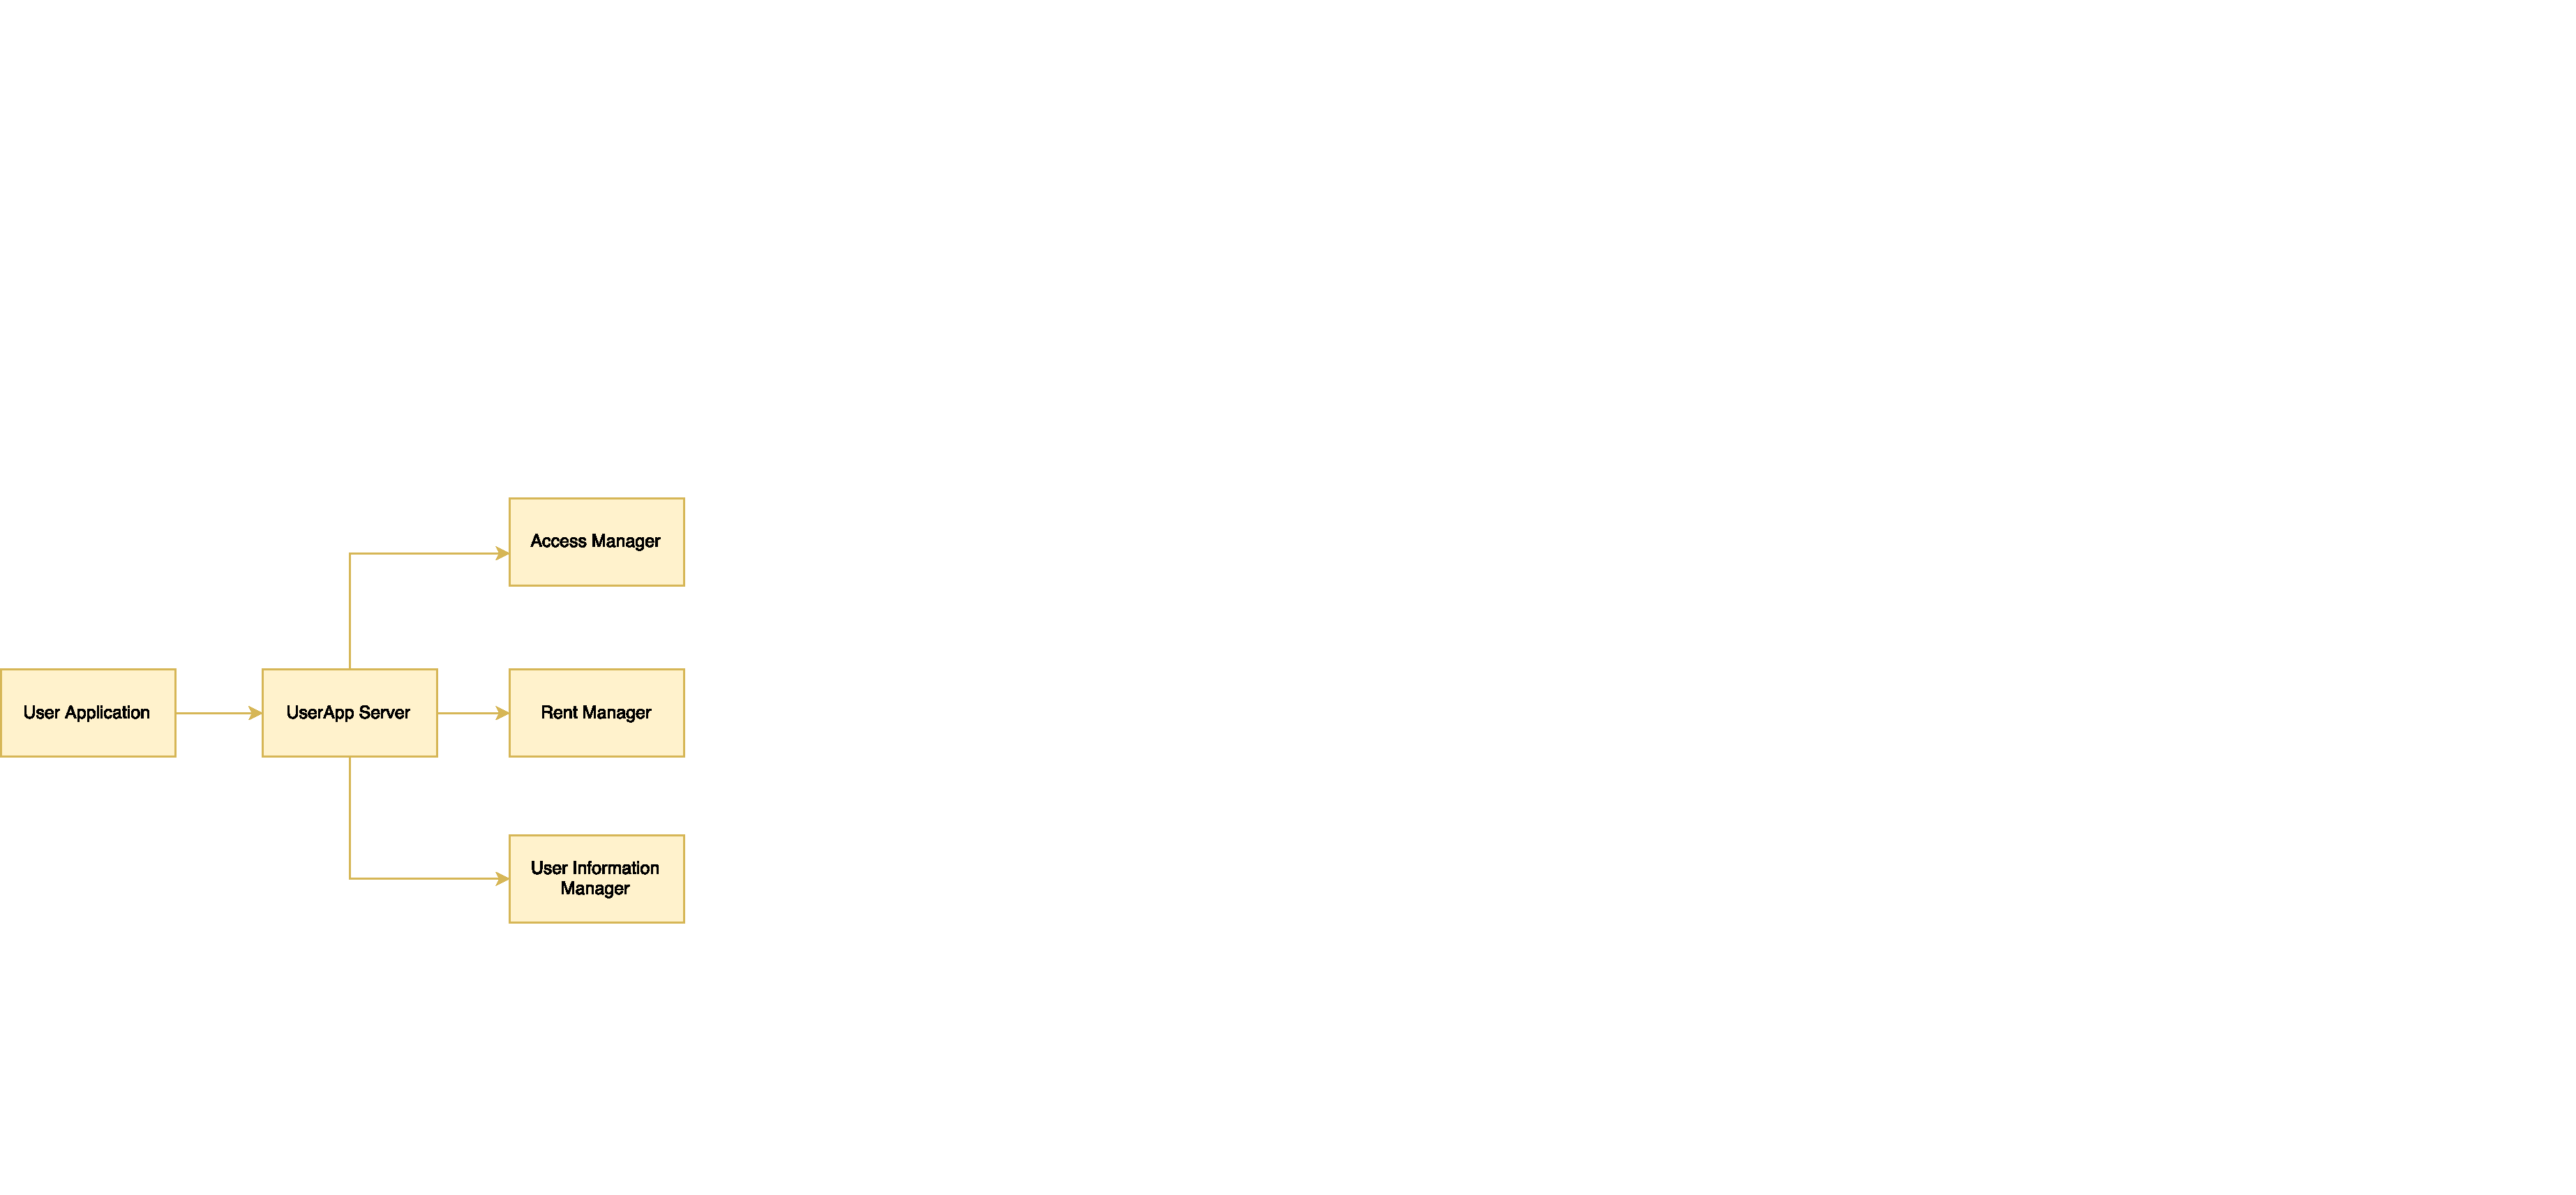
\includegraphics[width=0.7\linewidth]{img/Integration4}
			\caption{
				\label{fig:userAppServer} 
				\emph{User Application and Server integration}
			}
		\end{figure}
		
\paragraph{CustomerCare Application and Server} 
After that, we first integrate the \emph{CustomerCareServer} with the \emph{UserInformationManager} and the \emph{DataProvider} components  and secondly we test the integration between the \emph{CustomerCareApplication} and the \emph{CustomerCareServer} obtaining the complete test of the subsystem related to the functionalities provided to a customer care operator.
\paragraph{}
		
		\begin{figure}[h]
			\centering
			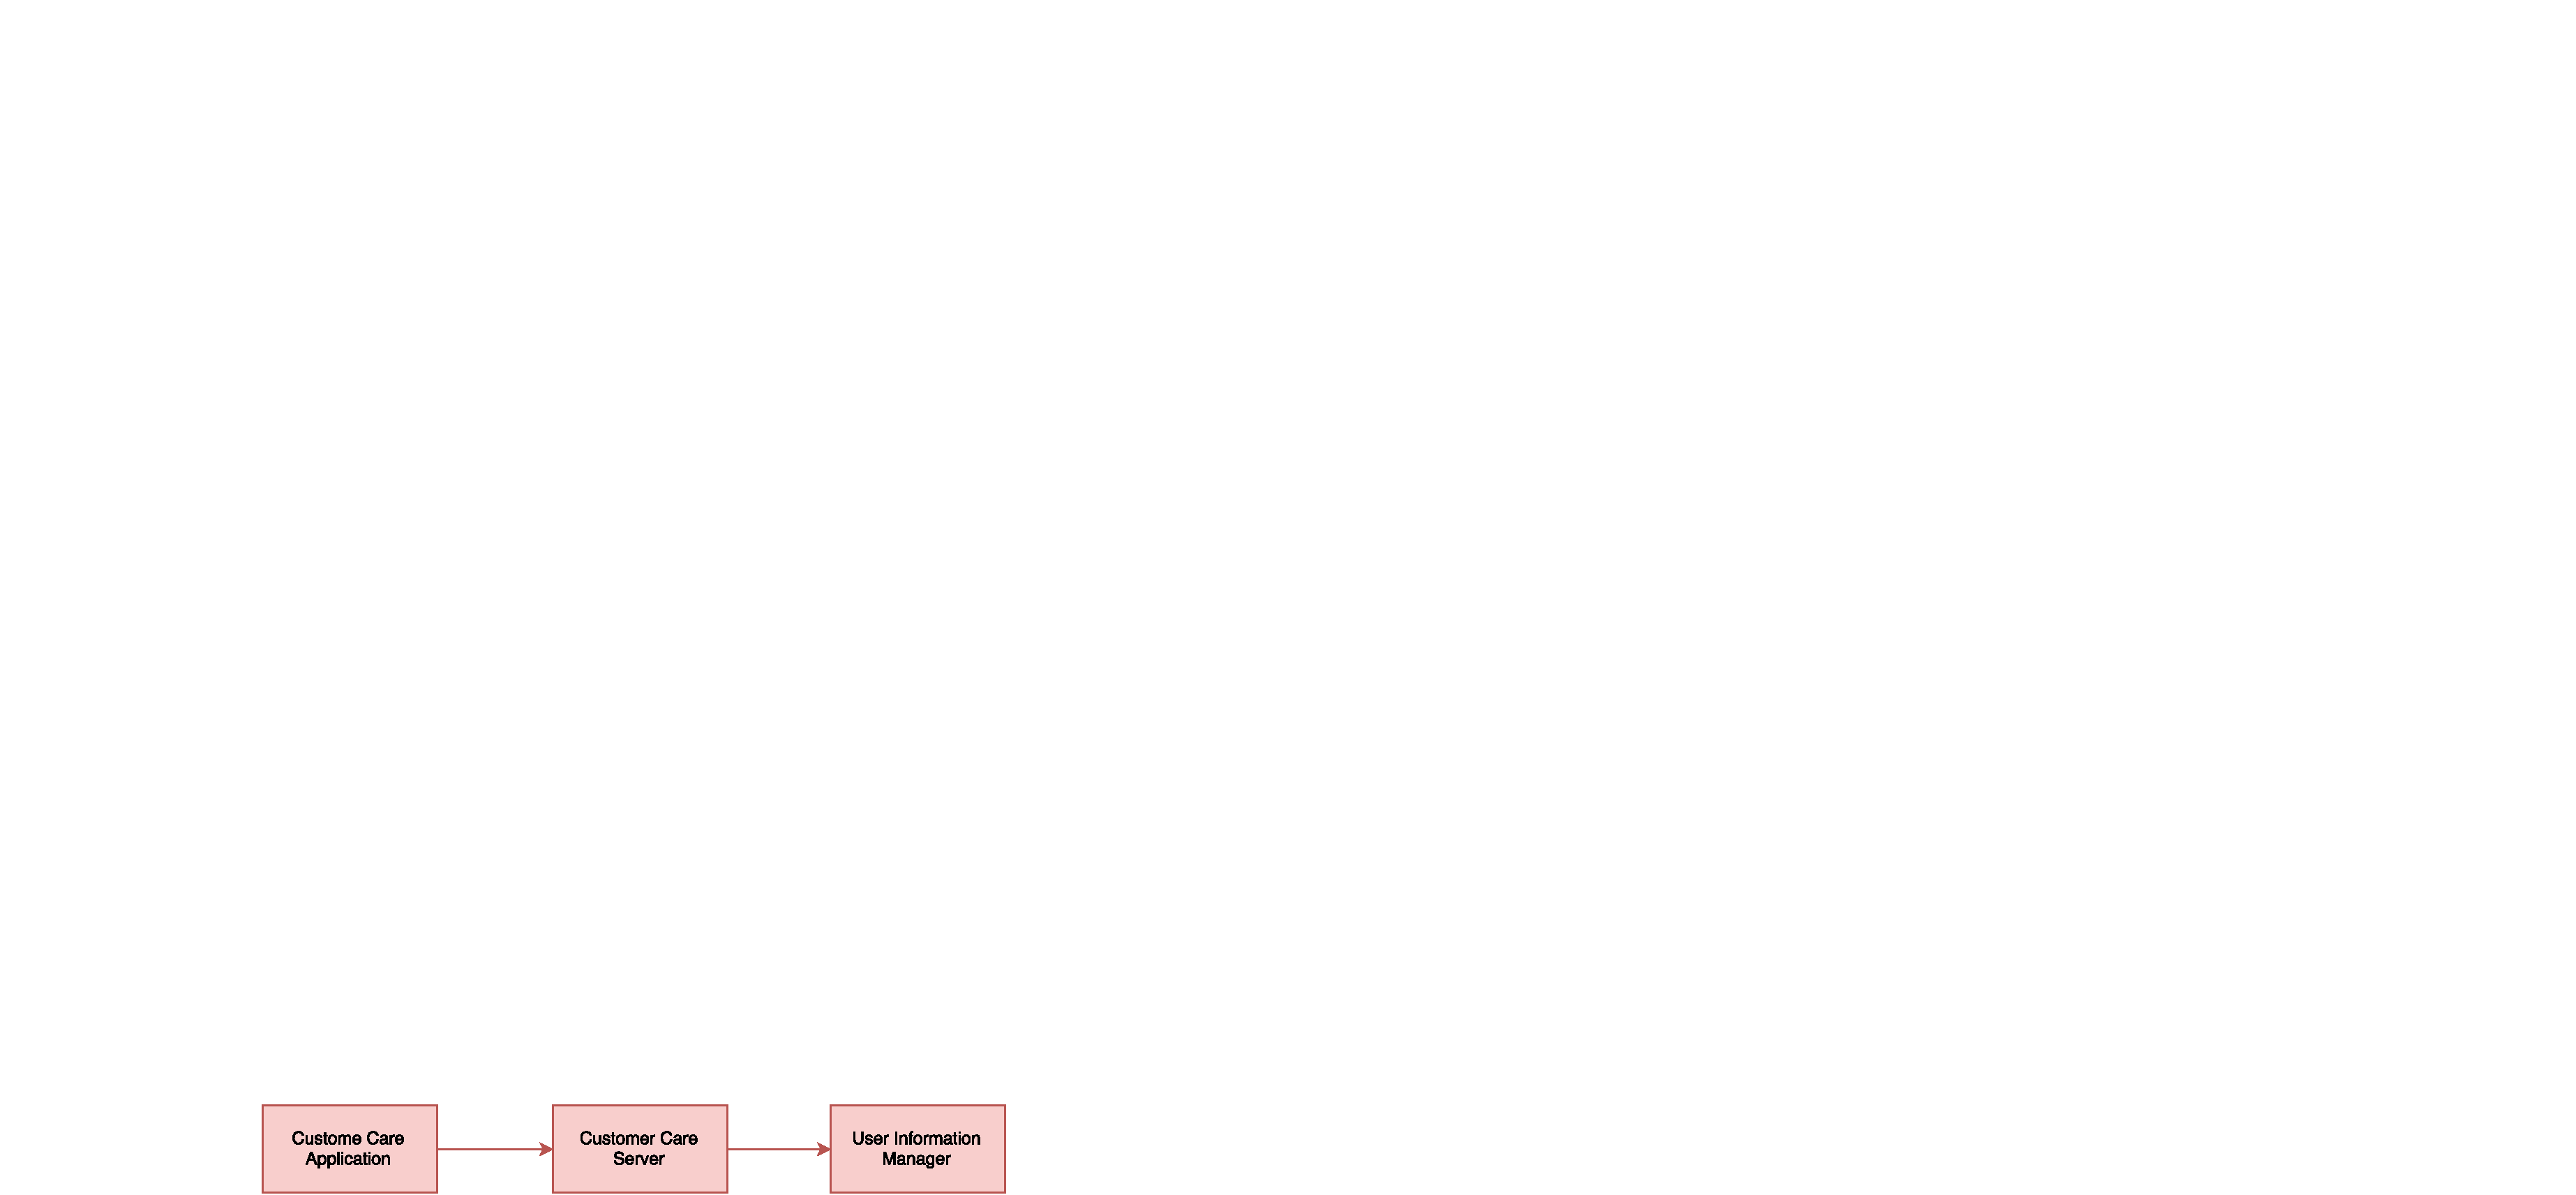
\includegraphics[width=0.8\linewidth]{img/Integration3c}
			\caption{
				\label{fig:ccAppServer} 
				\emph{CustomerCare Application and Server integration}
			}
		\end{figure}

\clearpage 

\subsubsection{Subsystem Integration Sequence}
Once the three major subsystem have been fully integrated and tested we integrate them together to test the whole system and its functionalities together; so we test the integration of the maintenance-related subsystem (figure \ref{fig:maintenanceManager}), the user-related subsystem (figure \ref{fig:userAppServer}) and the customer-care-related subsystem (figura \ref{fig:ccAppServer}).
This step may be split in different kind of tests on local machines but also on the real architecture we will use for our system in order to provide reliable test data also about performances and network issues.

	\begin{figure}[h]
			\centering
			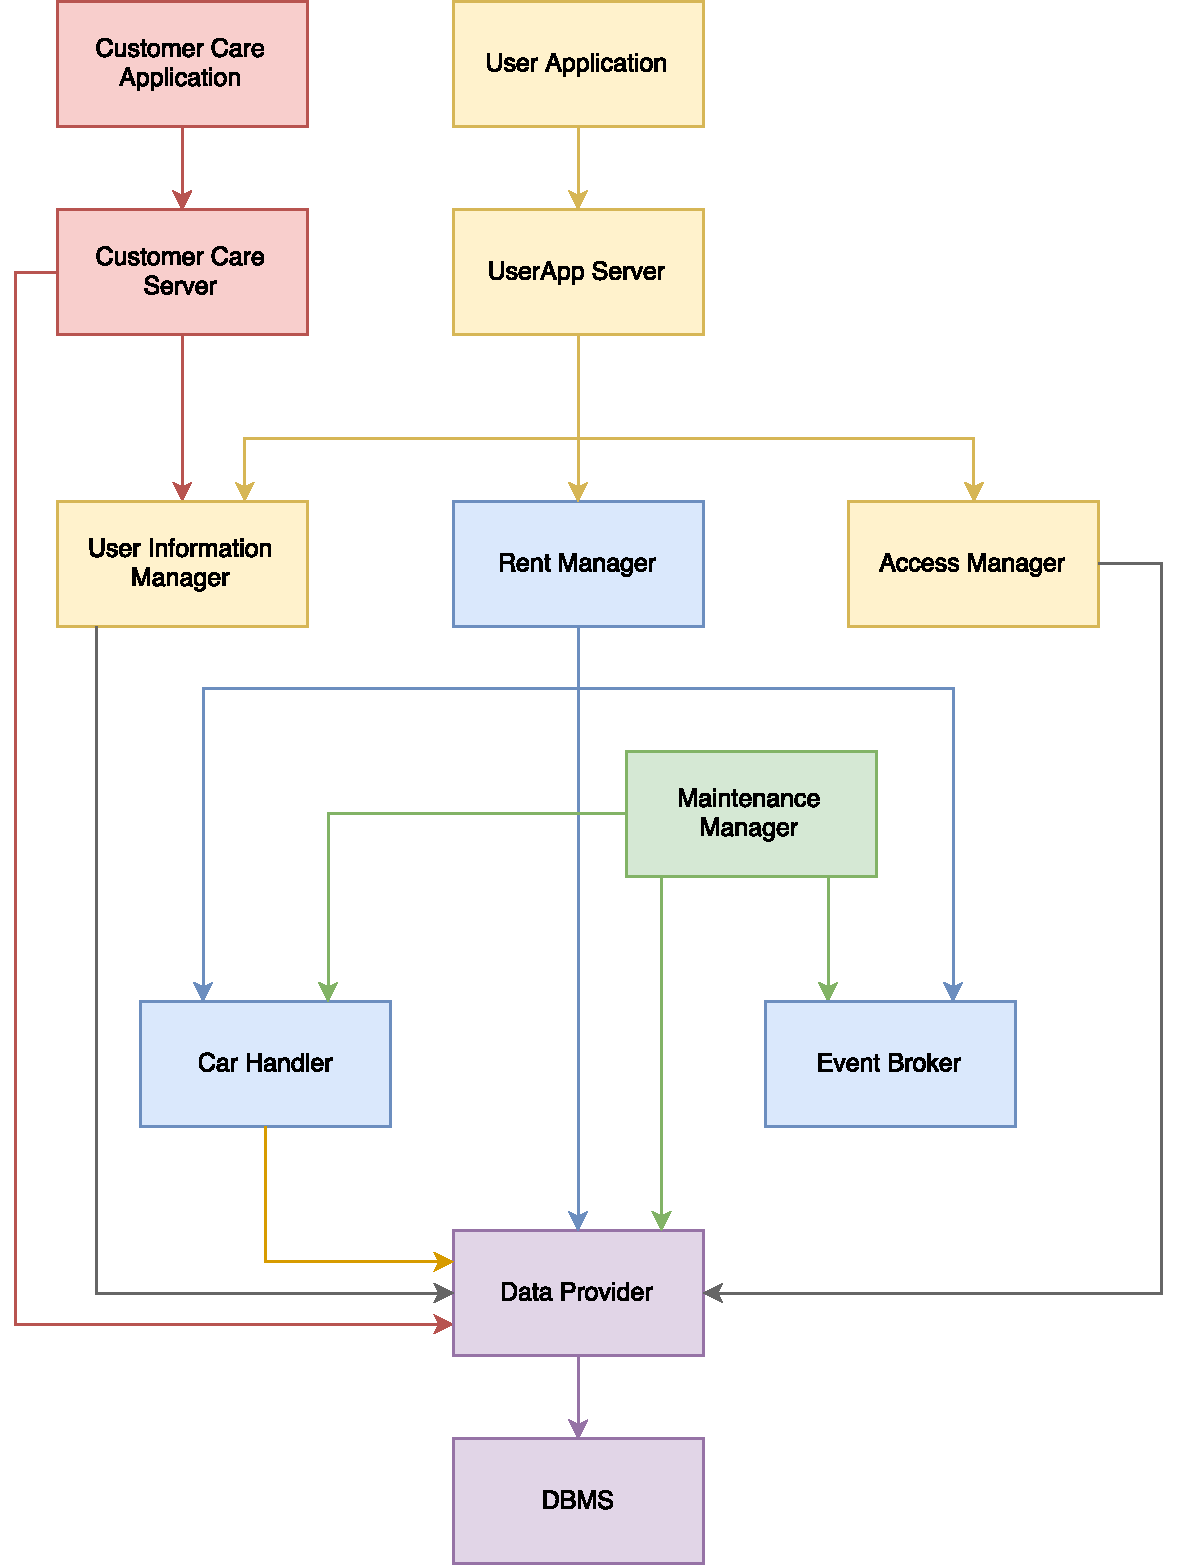
\includegraphics[width=0.7\linewidth]{img/subsystemIntegration}
			\caption{
				\label{fig:subsystemIntegration} 
				\emph{Subsystems Integration}
			}
		\end{figure}
